\documentclass[tikz,border=10pt]{standalone}
\usepackage{tikz}
\usetikzlibrary{arrows.meta, positioning}

\begin{document}

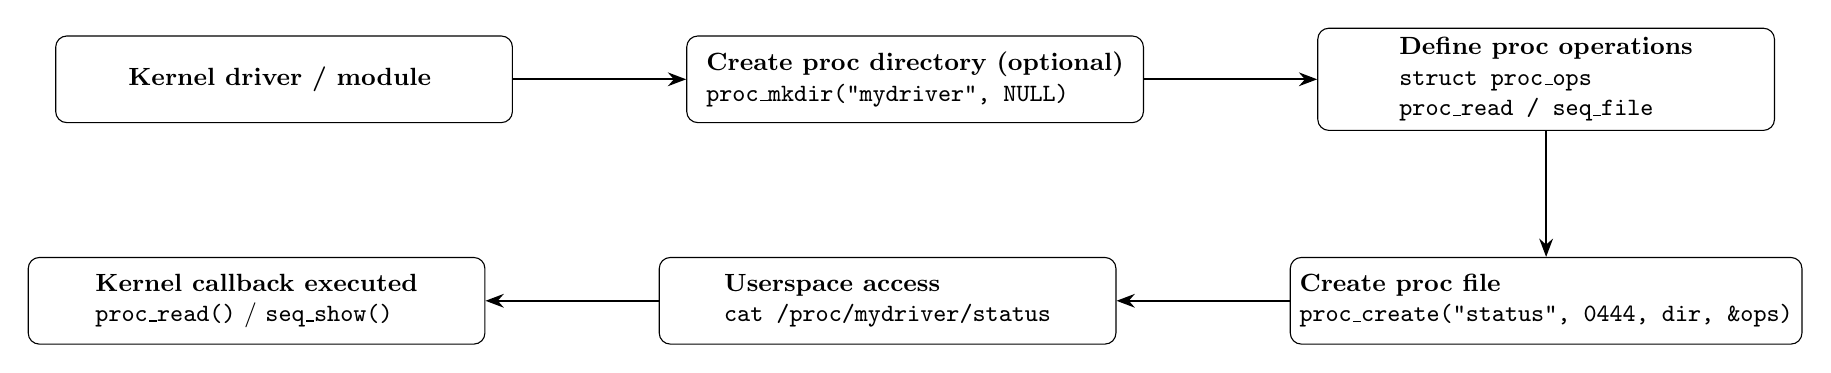
\begin{tikzpicture}[
    box/.style={
        draw,
        rounded corners,
        minimum width=5.8cm,
        minimum height=1.1cm,
        align=left,
        font=\small
    },
    arrow/.style={
        ->,
        thick,
        >=Stealth
    },
    node distance=1.6cm and 2.2cm
]

% ---------- Top row (left -> right) ----------
\node[box] (driver) {
    \textbf{Kernel driver / module}
};

\node[box, right=of driver] (mkdir) {
    \textbf{Create proc directory (optional)}\\
    \texttt{proc\_mkdir("mydriver", NULL)}
};

\node[box, right=of mkdir] (ops) {
    \textbf{Define proc operations}\\
    \texttt{struct proc\_ops}\\
    \texttt{proc\_read / seq\_file}
};

% ---------- Bottom row (right -> left) ----------
\node[box, below=of ops] (create) {
    \textbf{Create proc file}\\
    \texttt{proc\_create("status", 0444, dir, \&ops)}
};

\node[box, left=of create] (userspace) {
    \textbf{Userspace access}\\
    \texttt{cat /proc/mydriver/status}
};

\node[box, left=of userspace] (callback) {
    \textbf{Kernel callback executed}\\
    \texttt{proc\_read()} / \texttt{seq\_show()}
};

% ---------- Arrows ----------
\draw[arrow] (driver) -- (mkdir);
\draw[arrow] (mkdir) -- (ops);

\draw[arrow] (ops) -- ++(0,-0.9cm) -| (create);

\draw[arrow] (create) -- (userspace);
\draw[arrow] (userspace) -- (callback);

\end{tikzpicture}

\end{document}
